\documentclass{article}
%\usepackage[utf8]{inputenc}
\usepackage{graphicx, amsmath,amssymb,latexsym, booktabs,array,multirow}
\usepackage{listings}
%\usepackage[]{mcode}
\usepackage
[
        a4paper,% other options: a3paper, a5paper, etc
        left=2.54cm,
        right=2.54cm,
        top=1.5cm,
        bottom=1.8cm,
        % use vmargin=2cm to make vertical margins equal to 2cm.
        % us  hmargin=3cm to make horizontal margins equal to 3cm.
        % use margin=3cm to make all margins  equal to 3cm.
]{geometry}
\DeclareMathOperator*{\argmax}{argmax}
\title{Data Visualisation}
\author{ankitamehta }
\date{March 2017}

\usepackage{natbib}
\usepackage{hyperref}
\usepackage{graphicx}
\usepackage{tikz}
\begin{document}

\hrule height 1pt
\vspace{1em}
\begin{center}
\large{Data Visualisation(590V) - Project Report }\\
\large{Submitted by : Ankita Mehta }\\
\large{\href{http://www-edlab.cs.umass.edu/~amehta/}{Webpage Link}}
\end{center}
\par
\section*{Dataset Overview}
The dataset taken for this project has $48,842$ records with $15$ features. It is the adult dataset with size 5.3 MB, also knows as the "Census Income" dataset hosted by the UCI Machine Learning Repository. 
Here is the link from where it has been downloaded : https://archive.ics.uci.edu/ml/datasets/Adult/ \\

Dataset has following fields:
\begin{enumerate}
   \item Age            : Ordinal attribute denoting age of the person - Range from $17$ to $90$
     \item Workclass  : Nominal attribute denoting the working class of a person with values - Private, Self-emp-not-inc, Self-emp-inc, Federal-gov, Local-gov, State-gov, Without-pay, Never-worked.
   \item Fnlwgt        : Ordinal attribute denoting the survey weight - Range from $12285$ to $1490400$
   \item Education  :  Nominal attribute denoting the education level of a person with values - Bachelors, Some-college, 11th, HS-grad, Prof-school, Assoc-acdm, Assoc-voc, 9th, 7th-8th, 12th, Masters, 1st-4th, 10th, Doctorate, 5th-6th, Preschool. 
   \item Education-num : Ordinal attribute denoting the educational number given to each education level - Range from $1$ to $16$.
   \item Marital-status : Nominal attribute denoting the marital status of a person with values - Married-civ-spouse, Divorced, Never-married, Separated, Widowed, Married-spouse-absent, Married-AF-spouse.
   \item Occupation : Nominal attribute denoting occupation level of a person with values - ech-support, Craft-repair, Other-service, Sales, Exec-managerial, Prof-specialty, Handlers-cleaners, Machine-op-inspct, Adm-clerical, Farming-fishing, Transport-moving, 
   Priv-house-serv, Protective-serv, Armed-Forces. 
   \item Relationship : Nominal attribute denoting the relationship status of a person with values - Wife, Own-child, Husband, Not-in-family, Other-relative, Unmarried. 
   \item Race : Nominal attribute denoting race of a person with values - White, Asian-Pac-Islander, Amer-Indian-Eskimo, Other, Black. 
   \item Sex : Nominal attribute having two values - male or female.
   \item Capital-gain : Ordinal attribute denoting the capital gain contributed by the person - Range from $0$ to $99999$
   \item Capital-loss : Ordinal attribute denoting the capital loss caused by the person - Range from $0$ to $4356$
   \item Hours-per-week : Ordinal attribute denoting the total number of hours worked per week by the person - Range from $1$ to $99$
   \item Native-country : Nominal attribute denoting the country of origin of the person with values -  United-States, Cambodia, England, Puerto-Rico, Canada, Germany, Outlying-US(Guam-USVI-etc), India, Japan, Greece, South, China, Cuba, Iran, Honduras,    Philippines, Italy, Poland, Jamaica, Vietnam, Mexico, Portugal, Ireland, France, Dominican-Republic, Laos, Ecuador, Taiwan, Haiti, Columbia, Hungary, Guatemala, Nicaragua, Scotland, Thailand, Yugoslavia, El-Salvador, Trinadad \&Tobago, Peru,
  Hong, Holand-Netherlands. 
   \item Income : Nominal attribute having two values $>50k$ , $<50k$
\end{enumerate}

\noindent Various points that can be noticed here are as follows:
\begin{itemize}
\item Maximum records in this dataset are from United States.
\item There are many missing values in the dataset, denoted by ?. 
\item The Nominal values in the dataset has to be changed to ordinal to perform various Machine Learning techniques like classification, clustering, PCA.
\item It can also be noticed that educational-num and education attribute are giving the same information i.e the level of education of the person. For e.g: education-num 6 has been given to education level -10th and so on.
\item fnlwgt attribute can be ignored here, because it is not related anyhow to the other attributes.
\end{itemize}

\section*{Interest}  

I am interested in this dataset because of the following reasons:
\begin{itemize}
\item Firstly, the attributes/fields present in this dataset are related to daily life which makes it very easy to understand and work upon.
\item Secondly, this dataset has a very concrete goal i.e, whether the salary of the person is $>50k$ or $<50k$ and it has lot of records, so unsupervised and supervised machine learning techniques can be easily explored. Also it has 15 attributes, so Feature Selection and PCA can also be considered.
\item Thirdly, it has a geospatial attribute - Native Country, so Chloropleth visualisation can be explored for this project.
\end{itemize}

\noindent Various hypothesis that I answered about this dataset through my analysis are:
\begin{itemize}
\item What are the attributes upon which salary of a person is most-commonly dependent. Is the salary been affected by their race or marital-status etc. ? 
\subsubitem Answer to this hypothesis is that salary of a person is very much influenced by his sex, marital-status, education and occupation whereas race, number of hours worked and his age are not the influential factors while analysing the salary of an individual.
\item How are the factors like sex, education etc related to each other ?
\subitem Answer to this hypothesis has been given by using parallel coordinates visualisation technique - which is education and educational-num attributes are highly related to each other as they are conveying the same information. Whereas other attributes are not directly related to each other but collectively, say sex and education, are creating a great impact on the salary of an individual.
\item Which classifier has highest performance over this dataset : KNN , SVM etc.
\subitem This hypothesis is done to evaluate the analysis done about the dataset. It has been shown that an individual's income is highly impacted by the factors given by predicting this attribute using various classifiers. Random Forest performed the best on this dataset by predicting the salary of a person with $85 percent$  accuracy and acquiring 90 percent area under the Roc curve.
\item How does Principal Component Analysis performed on this dataset ?
\subitem As a part of evaluation of analysis, dimensions of given data are reduced to two. This has been done dynamically by choosing the attributes to include for PCA. It can be shown that persons salary is most affected by his education, marital-status, sex and occupation.
\end{itemize}

\section*{Analytics}  

Data is cleaned before processing in following ways :
\begin{itemize}
\item Firstly, Since dataset has around 48k records and around 3500 records has ? as missing values. So, these records can be deleted straightforward. 
\item Secondly, Nominal values needs to be changed to ordinal values to apply Machine Learning techniques and to make Parallel coordinates Visualisation. For an eg: $>50k$ and $<50k$ can be changed to $1$ and $0$ respectively.
\end{itemize}

\noindent Various analytical techniques that are applied here :
\begin{itemize}
\item Statistical information like Minimum/Maximum/Average are calculated for ordinal attributes in the dataset.
\item Classification techniques like SVM, KNN, Random Forest, Naive Bayes and Decision Trees have been applied and their performance haven been evaluated.
\item Dimensionality Reduction techniques like PCA has been explored.
\end{itemize}

\section*{Visualizations}  
Various Visualizations that will be explored for this dataset are :
\begin{enumerate}
\item {\textbf{Table}} having dataset information.
\item {\textbf{Grouped Barchart}} showing the division of records according to the specific attributes for salary $>50k$ and $<50k$. (For example :  $>50k$ and $<50k$ salary distribution for both male and female - sex attribute)
\item {\textbf{Scatterplot}} showing the relationship between nominal attributes(X-axis) and the ordinal attributes(Y-axis) with Income as the color attribute and also for PCA analysis
\item {\textbf{Pie Chart}} having percentage of samples according to various attributes.
\item {\textbf{Choropleth}} showing the world map with distribution of records in various countries.
\item {\textbf{Parallel Coordinates}} is used for showing the correlation between various features of this dataset.
\item {\textbf{Line chart}} is used for comparing the performance of various classifiers.
\item {\textbf{Bar chart}} is for comparing the performance of various classifiers.
\end{enumerate}

\section*{Interactions} 
 
Selection, Probing, Drop-down menu , Buttons, Checkboxes have been used wherever necessary.

\section*{Story}  

This project has explored the Adult income dataset by telling what are the main factors affecting the salary of a person. It has been done by analysing the dataset using various plots viz: grouped bar chart, scatterplot, pie-chart.
And then it has also been seen that if these attributes are related to each other or not. Then at the end, all the analysis done has been evaluated by applying various Machine Learning classifiers. It has been done to check which classifier performs the best or whether our analysis done is correct or not. It may be possible that salary of a person is not at all dependent on his/her education, sex , marital-status and we have done wrong predictions. As a part of evaluation, PCA has also been applied on the dataset, which is nothing but a dimensionality reduction technique. Using that one can see which all attributes when combined together can cluster the dataset into two parts effectively.

\section*{Implementation}  

Since dataset is bit large, loading webpage will take around 30-40sec. The last plot loaded will be Scatterplot for PCA. 
As you can see, there are four sections in the webpage:
\begin{itemize}
\item Firstly, the dataset has been explained - what are the factors that can affect the salary of an adult. Like - education, relationship, marital-status, sex, origin, race etc. Tables and world map have been made to describe the dataset.
\item Then three plots viz: Grouped bar chart, Pie chart and scatterplot have been made for analysing the affect of various factors described above. All these charts are interacting. ( On clicking any pie/bar of pie chart and grouped bar chart, respective area will be displayed in all the charts.) Drop-down menu has been provided to select the X and Y-axis for the charts. \\
Please have some patience while interacting with the charts, as they will take some seconds to filter.
\item In the next section, Parallel coordinates visualisation has been made which shows the correlation amongst the attributes described in 1st section. For this, nominal attributes have been mapped to the ordinal values which can be seen in the table. Attributes can be selected from the drop down menu.\\
Parallel coordinates are interactive in the sense that you can change the order of attributes by dragging and dropping. Specific points can be selected using the cursor over that axis.\\\\\\\\\\\\

You can find the visualisation like this after selection - \ref{fig:abc}

\begin{figure}[h]
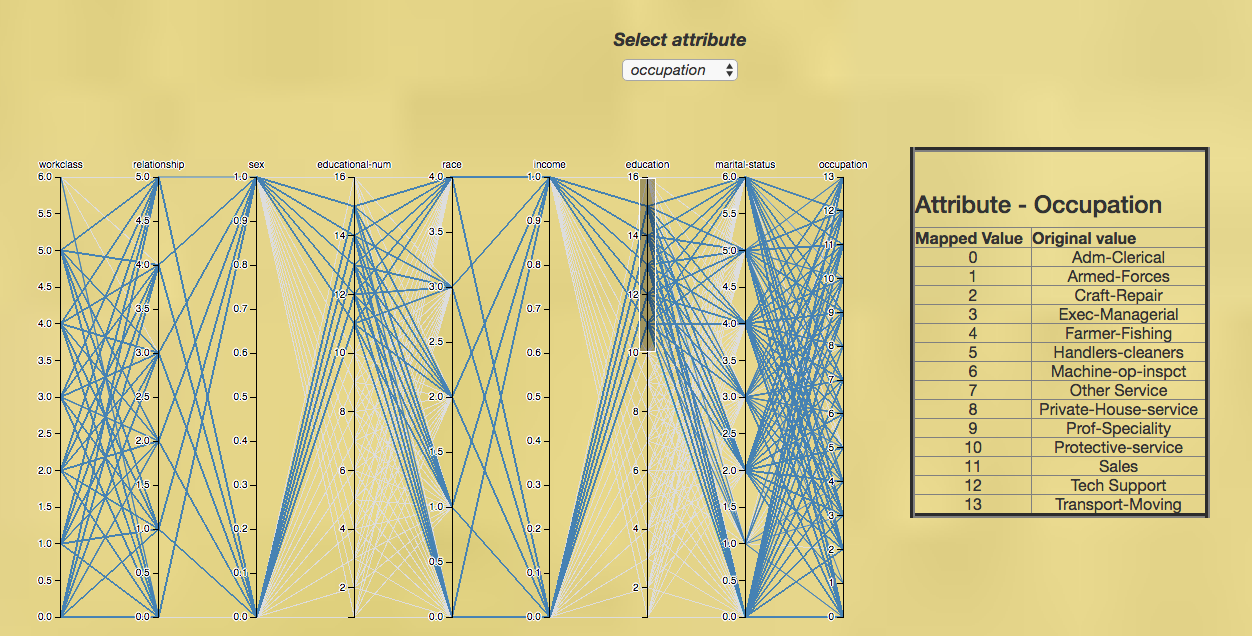
\includegraphics[scale=0.5]{abc.jpg}
\label{fig:abc}
\end{figure}

\noindent Interacting with this visualisation will take some time as filtering needs to be done over the large dataset.
\item Last section is for evaluating the analysis done using classification techniques like SVM, Random Forest, Decision Trees, Naive Bayes, KNN. Two plots viz: bar chart and line chart has been made for their performance analysis.
\item As a part of evaluation, scatterplot has been made to perform PCA dynamically. With the given checkboxes, you can select the attributes and check which set of attributes can cluster the dataset into two parts effectively. 

\end{itemize}


\section*{Previous work and WebPage Link}

The page referenced for the analysis of this dataset : \href{http://scg.sdsu.edu/dataset-adult_r/}{Previous work}\\

\noindent Link to the webpage for this project can be found at : \href{http://www-edlab.cs.umass.edu/~amehta/}{Project Link}

\end{document}

